\subsection*{Data Exploration}

\subsubsection*{Missing Values and Duplicates}
\begin{table}[H]
  \centering
  \begin{minipage}{0.48\textwidth}
    \centering
    \caption{Structure of the Ratings DataFrame}
    \label{tab:df-overview}
    \begin{tabular}{@{}ll@{}}
      \toprule
      Property      & Value                                             \\ 
      \midrule
      \# Rows       & 3{,}220{,}037                                     \\
      \# Columns    & 3 (\texttt{userID}, \texttt{profileID}, \texttt{rating})    \\
      Data types    & \texttt{int64}, \texttt{int64}, \texttt{int64}   \\
      Memory usage  & 73.7\,MB                                          \\
      \bottomrule
    \end{tabular}
  \end{minipage}%
  \hfill
  \begin{minipage}{0.48\textwidth}
    \centering
    \caption{Counts of Missing Values and Duplicate Rows}
    \label{tab:missing-dup}
    \begin{tabular}{@{}lrr@{}}
      \toprule
      Column         & Missing values & Duplicate rows \\ 
      \midrule
      \texttt{userID}    & 0              & 47                \\
      \texttt{profileID} & 0              & 0                 \\
      \texttt{rating}    & 0              & 0                 \\
      \bottomrule
    \end{tabular}
  \end{minipage}
\end{table}

\noindent\textbf{Unique entities.} After dropping duplicates, there are 25\,245 unique users and 125\,428 unique profiles.

\subsubsection*{Rating Distribution}
\begin{table}[H]
  \centering
  \caption{Descriptive Statistics of the \texttt{rating} Column}
  \label{tab:rating-stats}
  \begin{tabular}{@{}lrrrrrrrr@{}}
    \toprule
    Statistic & Count        & Mean   & Std    & Min & 25\% & 50\% & 75\% & Max \\ 
    \midrule
    Rating    & 3{,}220{,}037 & 5.9532 & 3.1064 & 1   & 3    & 6    & 9    & 10  \\
    \bottomrule
  \end{tabular}
\end{table}

\begin{figure}[H]
  \centering
  \begin{subfigure}[t]{0.348\textwidth}
    \centering
    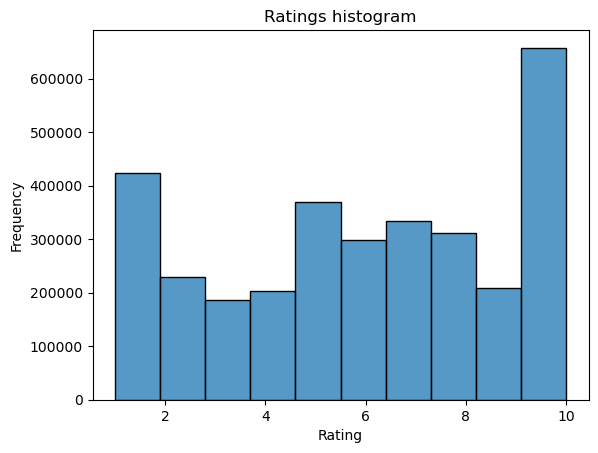
\includegraphics[width=\linewidth]{figures/hist.png}
    \caption{Histogram of Profile Ratings}
    \label{fig:hist-rating}
  \end{subfigure}
  \hspace{1cm}
  \begin{subfigure}[t]{0.34\textwidth}
    \centering
    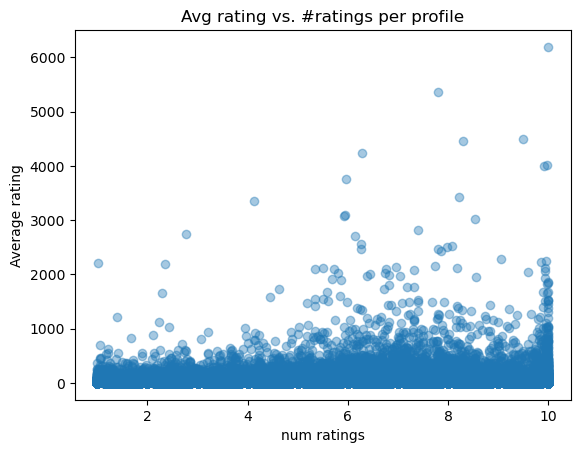
\includegraphics[width=\linewidth]{figures/output.png}
    \caption{Average Rating vs.\ Number of Ratings per Profile}
    \label{fig:rating-vs-count}
  \end{subfigure}
  \caption{(a) Distribution of all ratings; (b) Scatter of mean rating against count of ratings per profile.}
\end{figure}

\noindent\textbf{Figure \ref{fig:hist-rating}.} The histogram of all profile ratings reveals that the bulk of ratings lie between 3 and 9 on the 1–10 scale, with a slight concentration toward higher scores.  

\noindent\textbf{Figure \ref{fig:rating-vs-count}.} The scatter plot of average rating versus number of ratings per profile shows a diffuse cloud with no strong trend, indicating that a profile’s popularity does not necessarily correlate with higher or lower mean ratings.  

\subsubsection*{Profile Rating Frequency}
\begin{table}[H]
  \centering
  \caption{Statistics of Ratings Received per Profile}
  \label{tab:profile-stats}
  \begin{tabular}{@{}lrrrrrrrr@{}}
    \toprule
    Statistic        & Count     & Mean    & Std     & Min & 25\% & 50\% & 75\% & Max   \\ 
    \midrule
    \texttt{rating\_count} & 125\,428 & 25.6720 & 88.3126 & 1   & 2    & 7    & 21   & 6\,191 \\
    \bottomrule
  \end{tabular}
\end{table}

\subsubsection*{User Activity}
\begin{table}[H]
  \centering
  \caption{Number of Ratings Given per User}
  \label{tab:user-stats}
  \begin{tabular}{@{}lrrrrrrrr@{}}
    \toprule
    Statistic          & Count    & Mean    & Std     & Min & 25\% & 50\% & 75\%   & Max      \\ 
    \midrule
    \texttt{ratings\_given} & 25\,245  & 127.5496 & 362.0994 & 2   & 29   & 73   & 123    & 18\,342  \\
    \bottomrule
  \end{tabular}
\end{table}

\subsubsection*{Outlier Detection}
Using the IQR method ($Q_1 - 1.5\times\mathrm{IQR}$, $Q_3 + 1.5\times\mathrm{IQR}$), we found \textbf{0} outlier ratings, indicating no extreme anomalies.

\subsubsection*{Correlation Analysis}
The Pearson correlation between the number of ratings per profile and its average rating is
\[
  \mathrm{Corr}(\text{rating\_count},\,\text{avg\_rating})
  \;=\;0.0201,
\]
a very weak positive relationship, consistent with Figure~\ref{fig:rating-vs-count}.